\documentclass[conference]{IEEEtran} % onecolumn
\usepackage{cite}
\usepackage{amsmath,amssymb,amsfonts}
\usepackage{algorithmic}
\usepackage{graphicx}
\usepackage{textcomp}
\usepackage{xcolor}
\usepackage{float}
\usepackage{booktabs}
\usepackage{pxfonts}
\usepackage{listings}

\def\BibTeX{{\rm B\kern-.05em{\sc i\kern-.025em b}\kern-.08em
    T\kern-.1667em\lower.7ex\hbox{E}\kern-.125emX}}
    
% Define standard verbatim listing style
\lstdefinestyle{standard}{
  basicstyle=\fontsize{9}{9}\ttfamily,
  columns=flexible,
  breaklines=true,
  escapechar=\#
}

\begin{document}
\title{Generic Data Broadcast using Bluetooth Low Energy Advertisement Packets\\
}

\author{\IEEEauthorblockN{\textbf{David Jones}}
\IEEEauthorblockA{\textit{School of Electronics and Computer Science} \\
\textit{University of Southampton}\\
Southampton, United Kingdom \\
dsj1n15@ecs.soton.ac.uk}
\and
\IEEEauthorblockN{Richard Crosland}
\IEEEauthorblockA{\textit{School of Electronics and Computer Science} \\
\textit{University of Southampton}\\
Southampton, United Kingdom \\
rtc1g16@ecs.soton.ac.uk}
}
\maketitle

\begin{abstract}
Bluetooth is a ubiquitous communications technology present in billions of devices worldwide.



This article describes an approach for achieving offline and connectionless data broadcast using Bluetooth Low Energy (BLE) advertisement packets. 

The resulting protocol is fundamentally low-data rate but has high reliability and is unaffected by receiver count unlike a paired approach.
Although BLE is fundamentally low-power, the high duty-cycle used in the proposed solution makes this less true. 

\end{abstract}

\begin{IEEEkeywords}
BT, LE, BLE, Beacon, Broadcast, Lossy, Luby-Transform, Fountain Codes
\end{IEEEkeywords}

\section{Introduction}
Bluetooth\footnote{Bluetooth SIG, USA, https://www.bluetooth.com} is a short-range, single-hop communication technology, which as of 2019, is present in 100\% of shipped smartphones, tablets, and laptops \cite{BT:MARKET_RESEARCH}. Since 2010, implementations typically utilise Bluetooth v4.0 or newer; this packages Bluetooth Low Energy (BLE) alongside traditional (Classic) Bluetooth (BT) \cite{BT:CORE_SPEC}. This opens up mobile devices to proximity based content delivery services, such as: Apple's iBeacon\footnote{Apple, USA, https://developer.apple.com/ibeacon/}, Google's Eddystone\footnote{Google, USA, https://developers.google.com/beacons/eddystone} and and Radius Network's AltBeacon\footnote{Radius Network, USA, https://altbeacon.org}. These are used in many industries but are most prevalent in advertising for purposes such as tracking in-store shoppers \cite{BT:TRACK_USE_CASE} and delivering offers directly. Typically, content delivery implementations are backed by an internet server, allowing the beacon to transmit only a unique identifier (UUID) for which the target device can then download the corresponding payload. This allows beacons to operate completely offline and use minimal power, but limits deployments to locations where end-user's have a reliable internet connection. For purposes such as advertising, this connection would ideally be served by cellular LTE, though this can be unreliable indoors, whilst relying on users to connect to in-store Wi-Fi reduces potential catchment.

This article assesses whether small-medium payload broadcasting is viable using a BLE beacon approach without a second transfer medium. The use of fountain codes is explored as a way of coping with the unpaired lossy connection. A brief use case is also trialled using a custom data structure for generating offline advertisements.

\section{Background}
\subsection{Bluetooth Low Energy (BLE)}
As its namesake suggests, BLE has significantly lower power usage than BT to the point it can operate in an always-on fashion with minimal effect to the end-user -- the drawback being an overall lower achievable data-rate. This is achieved from a physical layer standpoint as well as the introduction of a simplified protocol stack; as shown in Figure \ref{fig:bt_stack}. 


\begin{figure}[H]
    \centering
   	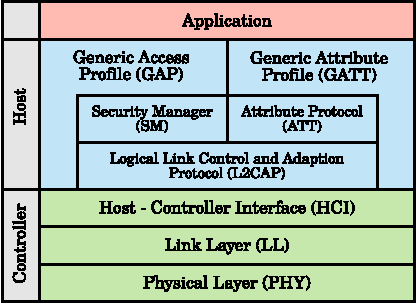
\includegraphics[scale=0.75]{Figures/bt_stack}
    \caption[Bluetooth network stack]{
  The BLE network stack adapted from [CITE]. 
    }
    \label{fig:bt_stack}
\end{figure}

Most BLE applications involve connecting multiple peripheral devices to a single device (the central), for example, connecting a heart-rate monitor and smartwatch to a mobile phone. This allows moderate one-to-one data transfer rates of approximately 125KB/s \cite{BT:LE_OVERVIEW}. These dedicated connection scenarios are handled by the Generic Attribute Profile (GATT). As communications that occur here are only visible by the intended receiver, broadcast is not possible. For sending small identical payloads to many receivers, this significantly increases network congestion and collisions associated with dense wireless environments. 

The Generic Access Profile (GAP) manages device advertisements and connections to nearby devices. Advertisements occur at frequent intervals or when a Scan Response Request is received from another device. Each Bluetooth Advertising Protocol Data Unit (PDU) has 31 bytes of data that can be set by the transmitter -- the rest being reserved for the BLE stack. By default these advertisements are sequentially transmitted to three BLE channels: 37 (2402MHz), 38 (2426 MHz), and 39 (2480 MHz). These channels are selected away from standard 2.4GHz Wi-Fi channels to reduce potential interference, giving higher receive probabilities than other BLE transmissions. Individual channels can be disabled to reduce power usage at the expense of receive probability. An advertisement can be either directed (unicast) or undirected (broadcast), and either connectable or non-connectable. Advertisements are the only place broadcast communications can occur and are the basis for beacon operation. As connecting defeats the purpose of broadcast behaviour, beacons are non-connectable. As specified by \cite{BT:CORE_SPEC}, non-connectable advertisements (\texttt{ADV\_NONCONN\_IND}) should be limited to transmission every 100ms unlike connectable advertisements (\texttt{ADV\_IND}) which can be sent every 20ms.



\subsection{BLE Beacons}
Although frame structures vary slightly and Eddystone beacons have some extra functionality, the fundamentals of all pre-mentioned beacon implementations are very similar. That is: periodically send BLE advertisements with some payload packaged in the manufacturer data section -- see Figure \ref{fig:altbeacon_frame} for AltBeacon's standard payload. An application on the receiver can interpret the data and perform relevant behaviour.


\begin{figure}[H]
    \centering
   	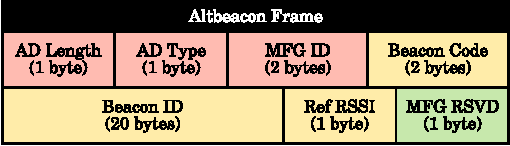
\includegraphics[scale=0.75]{Figures/altbeacon_frame}
    \caption[Altbeacon frame]{
  An AltBeacon frame. Note that 3 bytes of the manufacturer data are used to indicate that the advertisement is non-connectable and undirected hence making the maximum payload 28 bytes, not 31. Additionally, some fields are fixed. AD length is 0x1B (27) to indicate the payload size with AD Type set to 0xFF to indicate that the frame is manufacturer data and should not be handled by the stack. The Beacon Code is 0xBEAC to identify the frame as an AltBeacon. The rest of the fields values can change. The Manufacturer ID identifies the transmission hardware as per Bluetooth SIG company identifiers. The Beacon ID uniquely identifies the transmitter. The Reference RSSI is the received signal strength 1m away from the transmitter to allow for distance estimates. The Manufacturer Data is interpreted as defined by the Manufacturer ID but is generic. The manufacturer data is little endian whereas the rest is big endian. Adapted from [CITE].
    }
    \label{fig:altbeacon_frame}
\end{figure}

\section{Test/Development Infrastructure}
The testing and development platforms used for the findings of this article were as follows:
\begin{itemize}
	\item \textbf{Beacons:} Raspberry Pi 3's (Model B+) running Raspian OS; these have built-in BT v4.2 and the operating system provides BlueZ\footnote{BlueZ Project, http://www.bluez.org}, which directly exposes the Host-Controller Interface (HCI) as identified in Figure \ref{fig:bt_stack}. The command line tool was scripted using a Python wrapper.
	\item \textbf{End-devices:} Android smartphones, specifically the OnePlus X (BT v4.0) and Samsung S8 (BT v5.0). A bespoke application was developed with the Android Beacon Library\footnote{Radius Networks, USA, https://altbeacon.github.io/android-beacon-library/} providing the basis of BT interaction.
\end{itemize}

Beacon advertisements were set to occur at their fastest rate, every 100ms. The setup commands for BT were as follows (refer to \cite{BT:CORE_SPEC} for full command breakdowns):
\begin{lstlisting}[style=standard]
// Enable the BT interface
$ hciconfig up
// Disable scanning for other devices, transmit only
$ hciconfig noscan
// CMD : LE Set Advertising Parameters [p. 1321]
// (set to 100ms period) 
$ hcitool cmd 0x08 0x0006 A0 00 A0 00 03 00 00 00 00 00 00 00 00 07 00
// CMD : LE Set Advertising Enable [p. 1329]
// Enable non-connectable undirected advertising
$ hcitool cmd 0x08 0x000a 01
\end{lstlisting}
After setup, the periodically transmitted data could be set with the following command:
\begin{lstlisting}[style=standard]
// CMD : LE Set Advertising Data [p. 1326]
$ hcitool cmd 0x08 0x0008 {ADVERTISING_BYTES}
\end{lstlisting}

Likewise the Android Beacon Library was configured to receive as frequently as possible using a 50ms search period and 0ms between search periods.


\section{Advertisement Receive Testing}
To determine whether data broadcast using advertisement packets was viable, initial assessment of the receive probability for each packet was required. This was handled by sending typical AltBeacon frames with the Beacon ID holding a basic test payload -- the top 8 bytes set to a constant pattern that identifies test packets and the rest an incrementing packet identifier. The end-device reported the number of unique packets received as $n_{got}$. Tests transmitted 1000 packets ($n_{expected}$), after which an impression of receive probability could be gained ($n_{got} / n_{expected}$). The same packets were sent repeatedly until every unique packet had been received, $n_{repeats}$ giving  an indication of how many times a data payload would need to be retransmitted to ensure a single receiver gets the payload in the presence of no error correction. Of course, with the same packets being retransmitted, already received packets can be received again -- a clear waste of bandwidth. The results of performing the test 5 times are shown in Table \ref{tab:receive_prob}. An average receive probability of 53\% was found during the first transmission set with 9 repetitions required in the worst-case to receive all packets.

\begin{table}[htbp]
\caption{Test advertisment receive results}
\begin{center}
\begin{tabular}{c|ccccccccc}
\toprule
   & \multicolumn{9}{c}{\textbf{Repetition}} \\
\textbf{Test} & 1 & 2 & 3 & 4 & 5 & 6 & 7 & 8 & 9 \\
\midrule\addlinespace
1 & 556 & 834 & 960 & 992 & 998 & 998 & 999 & 999 & 1000 \\
2 & 440 & 796 & 944 & 987 & 999 & 1000 & - & - & -  \\
3 & 523 & 853 & 931 & 987 & 998 & 1000 & - & - & - \\
4 & 502 & 764 & 872 & 989 & 992 & 996 & 999 & 999 & 1000 \\
5 & 610 & 860 & 988 & 997 & 997 & 999 & 1000 & - & -  \\
\addlinespace\bottomrule
\end{tabular}
\end{center}
\label{tab:receive_prob}
\end{table}

\section{Proposal}
This article now proposes 

To avoid the high number of required repetitions 
As visibile in the test results, the channel is very lossy. Therefore 
A custom beacon format
to make throughput  a more viable amount 
When transmitting fast 
Doesn't work well with people dropping signal and getting it back

Clearly demonstrates a need for a form of error correction

Taking x
Having a second beacon transmitting the same pattern increased the receive count indicating that timing is the issue, not 


See how fast we can transmit, find some space in the packets, use some LubyTransform encoding, send some data, receive some data. Vwhola, dad's your uncle.


\section{Implementation}

\subsection{Encoding}

\subsection{Beacon Format}


\subsection{Payload}



To ensure compatibility with all beacon protocol types and beacon hardware, the manufactuer data is left intact.


Control from the Python side wrapping BlueZ hciconfig and hcitool commands 
Changing BLE frequency https://stackoverflow.com/questions/21124993/is-there-a-way-to-increase-ble-advertisement-frequency-in-bluez


Used lt-code Python library. Created separate encoder and decoder for handling reduced packet headers. 

No Java implementation so this was manually translated for Android application. Tested with individual component unit tests (from Python outputs).

Android side made use of a library AndroidBeaconLibrary. Android side also sped up from default. Implemented custom parsers for both test packets and data broadcasts. Test packets use standard AltBeacon structure with top 8 bytes of UUID a unique pattern and the lower part identifiying packet number (showing how many packets we get out of sent). Data packets we needed to get as much data as possible. Managed to get 21 bytes, but can filter out broadcast beacons to reduce chance of attempting to decode wrong data. First header identifies the chunk ID and a checksum so that you can verify that the data is actually a broadcast. The next header identifies the block seed, the amount of data needed for the file, and the block size. As block size would always be constant could save this byte. Maximum file size is 65500 bytes, more than would really be sensible to send at the low data rate.



The CRC higher in the BLE stack ensures the data received is valid.
If this CRC fails it is an indication that somehow a rogue packet has been incorproated into the decoding, or there is an invalid server-side implementation (PRNG is not generating the right shit)



\section{Viability}
Apple provides hardware acceleration for iBeacon's but no others.
- If constantly attempting to receive battery life will be awful
- Use of custom headers will mean hardware acceleration cannot be taken advantage of. One possible solution is to transmit standard infrequent iBeacon packets with the main data stream. These can trigger the receiver to go into strong receive mode. Using this method also gives the possibility of providing the otherwise removed power field for distance calculation.
The beacon can save power as people's devices will also transmit advertisments, so does not need to send anything until one is seen.

As indicated by \cite[p. 2178]{BT:CORE_SPEC} the advertisement wait period could be reduced provided the transmitter is silent when not required -- potentially increasing data-rate.


\section{Discussion}
It works. 40B/s is solid af.

\section{Conclusion}
Future work should be um, not doing this. It's dumb.
- Not really possible with iOS, needs to know which beacons it is attempting to receive

\bibliographystyle{IEEEtran}
\bibliography{IEEEabrv,mybibfile}

%\begin{thebibliography}{00}
%\bibitem{b1} Bluetooth SIG, \textit{``Bluetooth Market Update
%2019''}, White Paper, 2018
%\bibitem{b2} Bluetooth SIG, \textit{``Bluetooth Core Specification
%v5.1''}, White Paper, Bluetooth SIG, 21st January 2019
%\end{thebibliography}
\end{document}